\subsection{Login}
Wenn man die Applikation öffnet erscheinen zwei Eingabefelder (siehe Abb. \ref{fig:App_Login}), wobei beim oberen der Benutzername(die Novell-Schülernummer) und beim unteren das Passwort eingegeben werden muss. Der Punkt \enquote{angemeldet bleiben} kann ausgewählt werden, damit sich die Applikation beim nächsten Start selbst anmeldet. 


\begin{figure}[H]
\centering
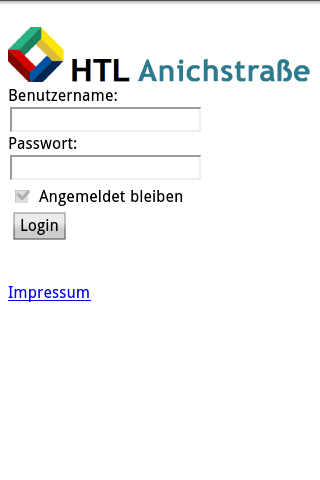
\includegraphics[keepaspectratio=true, width=7cm]{images/app_instructions/appLogin.png}
\caption{Loginbereich}
\label{fig:App_Login}
\end{figure}

\subsection{Menü}

Das Menü besteht aus drei Feldern (Stundenplan, Supplierplan und News), welche zur Weiterleitung zu den einzelnen Punkten wirken.

\begin{figure}[H]
\centering
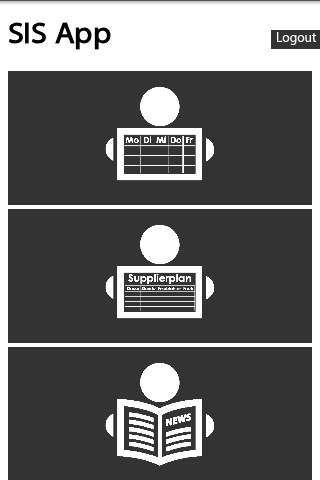
\includegraphics[keepaspectratio=true, width=7cm]{images/app_instructions/appMenu.png}
\caption{Hauptmenü}
\label{fig:App_Menu}
\end{figure}

\subsection{Stundenplan}
\subsubsection{Angepasster Stundenplan}
\label{sec:angepasster_stundenplan}
Um den für den Nutzer angepassten Stundenplan zu sehen, muss man im Menü das Stundenplansymbol antippen. In diesem Stundenplan ist der Supplierplan integriert, das heißt die Stunden werden so angezeigt, wie sie wirklich gehalten werden.\\
Es gibt die Möglichkeit den angepassten Stundenplan von dieser Woche oder von der nächsten Woche anzuzeigen, dazu gibt es rechts über der Tabelle einen Button auf dem steht, \enquote{nächste Woche} bzw. \enquote{vorherige Woche}.
Um weitere Informationen zu den einzelnen Stunden zu erfahren, kann man einfach auf die gewünschte Stunde tippen, daraufhin erscheint ein Popup, in welchem das Unterrichtsfach der genutzte Raum und der Lehrer/die Klasse aufgelistet sind.


\subsubsection{Normaler Stundenplan}
<<<<<<< HEAD
Um den gewöhnlichen Stundenplan zu sehen, muss man zuerst im Menü auf das Stundenplansymbol tippen, um zum angepassten Stundenplan zu gelangen und dann muss man auf den Schriftzug \enquote{normaler Stundenp.} am unteren Ende der Seite (siehe Abb. \ref{fig:App_Timetable_Bottom}) tippen, um zum normalen Stundenplan zu gelangen.\\
=======
Um den Standard Stundenplan zu sehen, muss man zuerst im Menü auf das Stundenplansymbol tippen, um zum angepassten Stundenplan zu gelangen und dann muss man auf den Schriftzug \enquote{normaler Stundenp.} am unteren Ende der Seite tippen, um zum normalen Stundenplan zu gelangen.\\
>>>>>>> f3465642d96ddd11a47a39927b2a34820107afa0
Um weiter Informationen zu den einzelnen Stunden zu erfahren, siehe \ref{sec:angepasster_stundenplan}

\begin{figure}[H]
\centering
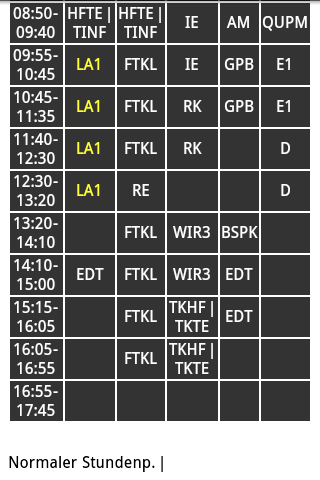
\includegraphics[keepaspectratio=true, width=7cm]{images/app_instructions/appTimetBottom.png}
\caption{Links zu weiteren Stundenplänen}
\label{fig:App_Timetable_Bottom}
\end{figure}

\subsubsection{Alle Stundenpläne}
Alle Stundenpläne (Klassenpläne) sind nur von Lehrern zu sehen. Um als Lehrer alle Stundenpläne einzusehen, muss man zuerst im Menü das Stundenplansymbol antippen, dann tippt man auf den Schriftzug \enquote{alle Stundenp.}, der neben dem Schriftzug \enquote{normaler Stundenp.}, am unteren Ende der Seite steht. Es erscheint ein Dropdownmenü.\\
In diesem Dropdownmenü muss man nun die Klasse auswählen, deren Stundenplan man sehen möchte und dann auf auswählen tippen. Nun erscheint der Stundenplan der ausgewählten Klasse.\\
Um weiter Informationen zu den einzelnen Stunden zu erfahren, siehe ~\ref{sec:angepasster_stundenplan}

\subsection{Supplierplan}
Im Supplierplan werden alle Supplierungen, die die eigene Klasse betreffen (wenn man als Lehrer angemeldet ist alle Supplierungen die einen selbst betreffen), angezeigt. Um diesen zu sehen, muss man im Menü auf das Supplierplansymbol tippen.\\
Um weitere Informationen zu den einzelnen Supplierungen zu erfahren, muss man auf ein Feld in der gewünschten Zeile tippen (leere Felder funktionieren nicht). Dann erscheint ein Popup, in welchem die zu supplierende Klasse, das Fach, der supplierende Lehrer und ein Kommentar stehen.

\subsection{News}
Bei den News werden immer die Neuigkeiten, welche auch auf den Monitoren ausgeschrieben werden,  angezeigt. Um zu den News zu gelangen, muss man im Menü auf den Menüpunkt News tippen.
